\documentclass[UTF8]{ctexart}
\usepackage{amsmath,amssymb}
\usepackage{tikz}
\usetikzlibrary{angles,quotes}
\begin{document}

% ============ 1 ============
\noindent \textbf{1.} 计算：
\[
|-2|-(\pi-3.14)^0+\left(\frac12\right)^{-2}-2\sin60^\circ-|\sqrt3-2|
\]
\begin{align*}
\text{原式}
&=2-1+4-2\cdot\frac{\sqrt3}{2}-(2-\sqrt3)\\
&=2-1+4-\sqrt3-2+\sqrt3\\
&=\boldsymbol{3}
\end{align*}

\vspace{4mm}
% ============ 3 ============
\noindent \textbf{3.} 已知 $\alpha$ 是锐角，且 $\tan\alpha=3$，求
$\dfrac{\sin\alpha+\cos\alpha}{\sin\alpha-\cos\alpha}$ 的值。
\begin{align*}
\frac{\sin\alpha+\cos\alpha}{\sin\alpha-\cos\alpha}
&=\frac{\dfrac{\sin\alpha}{\cos\alpha}+1}
{\dfrac{\sin\alpha}{\cos\alpha}-1}
\quad\text{（分子分母同除以 $\cos\alpha$）}\\
&=\frac{\tan\alpha+1}{\tan\alpha-1}\\
&=\boldsymbol{2}
\end{align*}

\vspace{4mm}
% ============ 6 ============
\noindent \textbf{6.} 构造图形求 $\tan15^\circ$。

在 Rt$\triangle ABC$ 中，$\angle C=90^\circ,\ \angle B=30^\circ$，设 $AC=1$，
则 $BC=\sqrt3,\ AB=2$。

\begin{center}
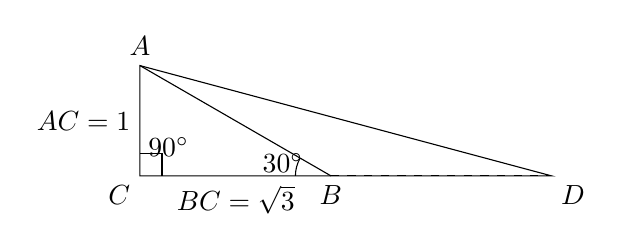
\begin{tikzpicture}[scale=1.4]
\coordinate (C) at (0,0);
\coordinate (A) at (0,1);
\coordinate (B) at (1.732,0);
\coordinate (D) at (3.732,0);

\draw (A)--(C)--(D)--cycle;
\draw (A)--(B);
\draw[dashed] (B)--(D);

\node[above] at (A) {$A$};
\node[below left] at (C) {$C$};
\node[below] at (B) {$B$};
\node[below right] at (D) {$D$};

\node[left] at (0,0.5) {$AC=1$};
\node[below] at (0.87,0) {$BC=\sqrt3$};

\draw pic[draw, angle radius=0.28cm, "$90^\circ$",
          angle eccentricity=1.3] {right angle=B--C--A};
\draw pic[draw, angle radius=0.45cm, "$30^\circ$",
          angle eccentricity=1.4] {angle=A--B--C};
\end{tikzpicture}
\end{center}

$\triangle ABD$ 为等腰三角形：
\[
\angle ABD=180^\circ-30^\circ=150^\circ
\Rightarrow \angle D=\angle BAD=\frac{180^\circ-150^\circ}{2}=15^\circ
\]
\begin{align*}
\tan15^\circ&=\frac{AC}{CD}=\frac{1}{2+\sqrt3}
=\frac{2-\sqrt3}{(2+\sqrt3)(2-\sqrt3)}\\
&=\boldsymbol{2-\sqrt3}
\end{align*}

\end{document}
